\documentclass[main.tex]{subfiles}

\begin{document}
\section{Without \starpu} \label{sec:prof:cpu}

\subsection{\cpu}

For the \cpu implementation, earlier analyzis of the original implementation relatively bad scalability. The actual results are not presented here due to different algorithms being employed (profiling of original version was done only on PPM version and not SPPMPA), and no assumptions could be made about code quality, as explained in \cref{section:impl_original}.
Instead, a scalability analyzis was made on the actually implemented \cpu version, shown in \cref{fig:prof:cpu}.

\begin{figure}[!htp]
  \centering
  \begin{subfigure}{.5\textwidth}
    \centering
    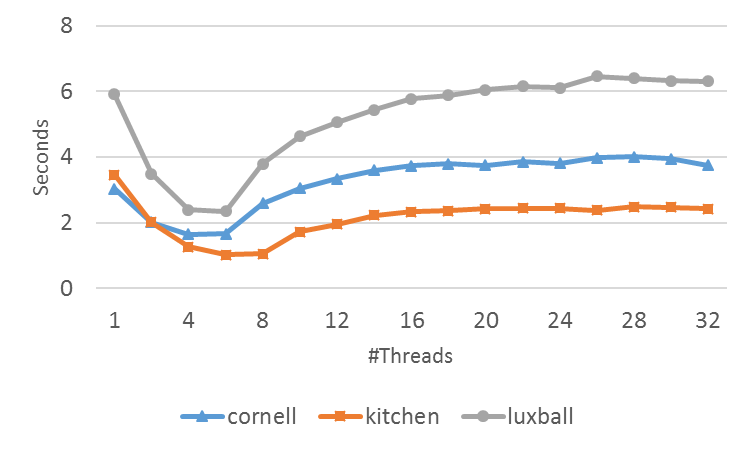
\includegraphics[width=\linewidth]{profiling/cpu_time}
    \caption{Avg iteration time \label{fig:prof:cpu_time}}
  \end{subfigure}%
  \begin{subfigure}{.5\textwidth}
    \centering
    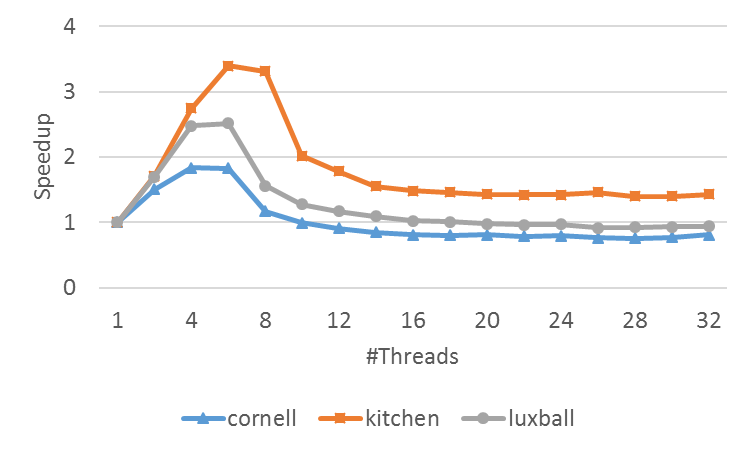
\includegraphics[width=\linewidth]{profiling/cpu_speedup}
    \caption{Speedup vs sequential version \label{fig:prof:cpu_speedup}}
  \end{subfigure}
  \caption{\cpu implementation \label{fig:prof:cpu}}
\end{figure}

It can be seen that good scalability is achieved only until around 6 threads are reached, which is more or less the point at which a single \cpu socket is filled, at which point performance starts to degrade.
For \textbf{luxball} and \textbf{cornell} scenes, performance with 16 threads (same amount as physical \cpu cores in the test machine) actually barely differs from the sequential approach.

The end conclusion is that scalability is only good when a single socket is used. The algorithm is clearly memory bounded, especially considering the fact that the test machine uses a \acs{NUMA} architecture. This pins all memory allocated by the master thread (such as the input scene, which is heavily used throughout the algorithm) to one of the sockets, leaving the other with slower access times to such memory.

Memory affinity tools such as \texttt{hwloc} could prove useful here, for example, by creating multiple copies of the input scene, and pinning each one to each \acs{NUMA} node. Each socket would then benefit from faster accesses to its own memory node.

\subsubsection{\cuda}

When analyzing the \gpu implementation, tests were made on both available \gpus, and compared against the base sequential \cpu implementation. The best execution time on \cpu was also included for comparison.

It should be taken into account that, as explained before, this is not a full-\gpu implementation, requiring in-loop memory transfers, and some \cpu computation to generate the lookup table. Since this was not implemented on \gpu, it should add a considerable overhead to the execution. Still, \cref{fig:prof:cuda} shows the implementation is able to outperform the \cpu in two of the three cases, achieving a speedup of around 3 when compared to the sequential approach.

\begin{figure}[!htp]
  \centering
  \begin{subfigure}{.5\textwidth}
    \centering
    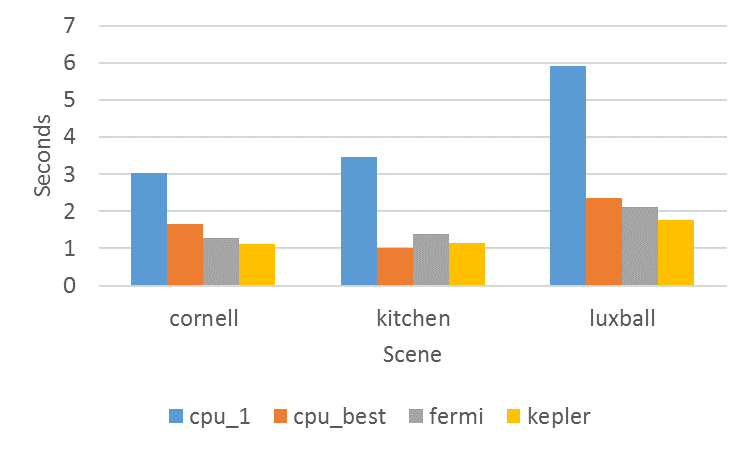
\includegraphics[width=\linewidth]{profiling/gpu_time}
    \caption{Avg iteration time \label{fig:prof:cuda_time}}
  \end{subfigure}%
  \begin{subfigure}{.5\textwidth}
    \centering
    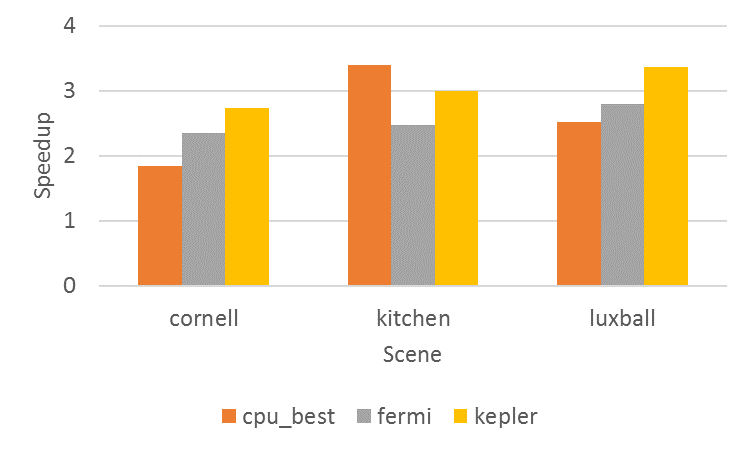
\includegraphics[width=\linewidth]{profiling/gpu_speedup}
    \caption{Speedup vs sequential version \label{fig:prof:cuda_speedup}}
  \end{subfigure}
  \caption{\cuda implementation \label{fig:prof:cuda}}
\end{figure}
\end{document}
